\chapter{KONSEP PERANCANGAN}
\label{BAB3:Metode}
\section{Diagram Alir Perancangan}
Perancangan sistem dilakukan dalam beberapa tahap untuk menghasilkan sistem 
yang dapat bekerja dengan baik saat melakukan diagnosis indeks kesehatan pada 
transformator daya. Pada Gambar \ref{gambar:diagram alir} merupakan tahapan perancangan yang 
digambarkan dalam diagram alir
\begin{figure}[h]
	\begin{center}
		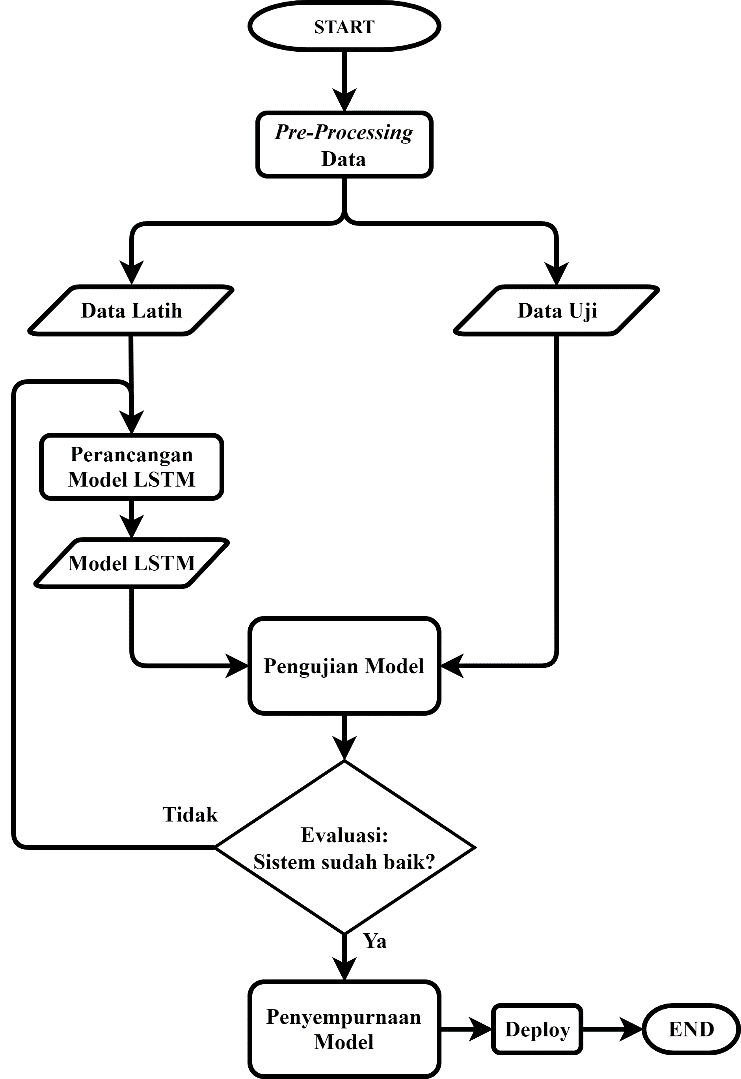
\includegraphics[width=0.7\textwidth]{BAB-3/figures/diagram alir.png}	
		\caption{Diagram Alir Perancangan Sistem Model LSTM}
		\label{gambar:diagram alir}
	\end{center}
\end{figure}

\section{Pertimbangan Perancangan}
Pada perancangan ini pertimbangan utama penggunaan model LSTM adalah karena pada dasarnya LSTM mampu memprediksi suatu klasifikasi dimana vektor masukan (\textit{input}) yang diberikan akan saling mendukung. Dalam diagnosis indeks kesehatan transformator daya prosesnya dilakukan melalui beberapa hasil pengujian yang berupa pengujian kimia, fisik, maupun elektrik. Data hasil pengujian pada dasarnya saling berkaitan, misalnya pengujian tegangan tembus erat kaitanya dengan adanya kontaminasi pada bahan dielektrik, di sisi lain pengujian secara kimia dilakukan dengan menggunakan DGA untuk mengetahui kandungan gas yang terlarut. Pada proses pembuatan model LSTM \textit{input} yang akan digunakan nantinya adalah data hasil percobaan pengujian transformator daya. Merujuk pada sifat model LSTM yang mengingat semua \textit{imput} untuk mendapatkan hasil prediksi yang maksimal, maka penggunaan model ini memiliki kecocokan terhadap proses diagnosis indeks kesehatan transformator daya. \par 


Menggunakan metode LSTM dalam memodelkan diagnosis indeks kesehatan transformator tidak dapat dilakukan secara langsung. Pemodelan harus disesuaikan dengan sistem yang akan diterapkan. Oleh karena itu akan dilakukan beberapa percobaan untuk memodifikasi arsitektur pada LSTM. Terdapat beberapa pertimbangan utama dalam menentukan baik dan tidaknya suatu model dapat dilakukan dengan melihat performa dari sistem tersebut. Performa sistem pada algoritma machine learning umumnya dapat ditentukan dengan menggunakan confusion matrix. Dari confusion matrix selanjutnya akan diperoleh akurasi, presisi, sensitifitas, specificity, dan F1 score.
 
\begin{table}[h]
	\centering
	\caption{\textit{Confussion Matrrix}}
	\label{tabel::Conf Matrix}
	\begin{tabular}{|c|c|c|c|} 
		\hline
		\multicolumn{2}{|c|}{\multirow{2}{*}{\begin{tabular}[c]{@{}c@{}}Confussion\\Matrix\end{tabular}}} & \multicolumn{2}{c|}{Nilai Aktual}                            \\ 
		\cline{3-4}
		\multicolumn{2}{|c|}{}                                                                            & \multicolumn{1}{l|}{Positif} & \multicolumn{1}{l|}{Negatif}  \\ 
		\hline
		\multirow{2}{*}{\rotcell{\begin{tabular}[c]{@{}c@{}}Nilai\\Terprediksi\end{tabular}}} & Positif   & TP                           & FP                            \\ 
		\cline{2-4}
		& Negatif   & FN                           & TN                            \\
		\hline
	\end{tabular}
\end{table}

\subsection{Akurasi}
Nilai akurasi menunjukkan seberapa akurat dalam memprediksi suatu nilai. Dalam 
confusion matrix akurasi merupakan rasio prediksi Benar (positif dan negatif) 
dengan total keseluruhan data. Algoritma machine learning dipilih berdasarkan 
akurasi yang tinggi jika dataset yang digunakan memiliki jumlah data False 
Negative (FN) dan False Positive (FP) yang sangat mendekati (symmetric).

\subsection{Presisi}
Nilai dari presisi merupakan perbandingan data yang terprediksi benar yang 
bernilai positif terhadap keseluruhan jumlah data yang bernilai positif dan 
yang bernilai negatif. Pemilihan nilai presisi sebagai bahan pertimbangan 
dalam 
menentukan model yang terbaik jika diinginkan terjadinya prediksi benar yang 
bernilai positif, serta sangat menghindari terjadinya hasil prediksi yang 
salah 
dan bernilai negatif. 

\subsection{Sensitifitas (\textit{recall})}
Sensitifitas merupakan perbandingan data yang terprediksi benar yang bernilai 
positif dibandingkan terhadap keseluruhan data yang terprediksi benar dan 
bernilai positif. Pertimbangan pemilihan nilai ini diambil jika model yang 
diinginkan merupakan model yang memiliki kecenderungan memprediksi salah 
bernilai positif dibandingkan dengan hasil prediksi salah yang bernilai 
negatif.

\subsection{Spesificitiy}
Specificity merupakan perbandingan antara data yang terprediksi dengan benar 
yang bernilai negatif terhadap keseluruhan data yang bernilai negatif. 
Pemilihan nilai ini didasarkan jika model tidak diinginkan terjadinya hasil 
prediksi yang bernilai positif.

\subsection{\textit{F1 Score}}
F1 Score merupakan perbandingan rata-rata dari presisi dan recall yang dilakukan pembobotan. Nilai dari F1 Score dijadikan sebagai pertimbangan baik dan tidaknya suatu algoritma machine learning jika nilai dari nilai dari hasil prediksi salah dengan nilai negatif (FN) dan False positif (FP) berbeda jauh.

\subsection{Waktu Pelatihan dan Pengujian}
Waktu training merupakan durasi waktu yang dibutuhkan dalam proses pelatihan untuk mendapatkan nilai performa tertinggi dalam satu data set. Waktu testing merupakan waktu yang dibutuhkan dari suatu sistem dalam memprediksi dari \textit{input} yang belum pernah di berikan pada sistem. Kedua parameter ini dapat dijadikan acuan sebagai baik dan buruknya suatu sistem biasanya untuk waktu pemrosesan  yang lebih singkat tidak dibutuhkan komputasi yang besar sehingga spesifikasi hardware yang digunakan tidak terlalu tinggi.

\section{Perancangan Model LSTM}

Sistem diagnosis indeks kesehatan transformator daya yang diharapkan pada dasarnya adalah yang memiliki performa yang baik. Sehingga pada perancangan ini dilakukan percobaan untuk mendapatkan model dari LSTM dengan akurasi minimal 85\% baik pada proses pelatihan dan pengujian. Indikator yang digunakan dalam penilaian baik dan buruknya sistem adalah nilai \textit{loss} serta akurasi sistem. Nilai \textit{loss} terbaik adalah yang minimum, sedangkan akurasi ditentukan yang terbesar. Untuk mendapatkan model dengan performa yang diharapkan baik dilakukan beberapa modifikasi pada arsitektur pada LSTM diantaranya jumlah \textit{neuron} pada setiap sel serta penggunaan banyaknya \textit{layer} LSTM yang digunakan. Di sisi lain perlakukan pada pembagian dataset juga menjadi fokus pembahasan pada perancangan.

\subsection{Jumlah \textit{Neuron}}
Model LSTM pada dasarnya merupakan pengembangan dari algoritma \textit{Neural Network} sehingga jumlah neuron akan mempengaruhi kapasitas belajar jaringan. Secara umum, lebih banyak neuron akan dapat mempelajari lebih banyak struktur dari dataset namun konsekuensinya akan membutuhkan waktu pelatihan yang lebih lama. Kapasitas belajar yang lebih besar juga menimbulkan masalah kemungkinan \textit{overfitting} pada data pelatihan sehingga akan sensitif terhadap adanya data yang memiliki \textit{noise}.

\subsection{\textit{Multilayer layer} LSTM}
Jumlah \textit{layer} LSTM secara umum digunakan dalam meningkatkan performa sistem karena secara sederhana jika pada penggunaan \textit{single layer} nilai prediksi hanya mempertimbangkan masukan masing-masing sel serta keluaran hanya ditentukan oleh sel terakhir. Pada penggunaan \textit{multilayer} keluaran akhir sistem akan mempertimbangkan keluaran setiap sel pada layer sebelumnya. Penambahan \textit{layer} LSTM akan menambah kapasitas belajar dari model yang akan membuat proses pelatihan cenderung lebih lama. Sehingga pada perancangan penambahan \textit{layer} tidak dilakukan pada jumlah yang banyak agar sistem cepat dalam hal komputasi namun performa masih memiliki akurasi yang tinggi. 

\subsection{Rasio Dataset}
Pada proses pelatihan dan pengujian pada \textit{machine learning} jumlah dataset yang digunakan dapat mempengaruhi performa sistem. Semakin banyak jumlah dataset yang digunakan dalam proses pelatihan secara ideal dapat memperbaiki performa karena model dapat terlatih dengan banyaknya data. Namun disisi lain dalam proses validasi diperlukan sebagian dari dataset untuk menguji sistem ketika dihadapkan pada data yang belum pernah dikenali. Sehingga diperlukan rasio yang tepat agar model yang dihasilkan memiliki performa yang baik pada proses pelatihan dan pengujian. Pada perancangan ini akan dilakukan beberapa percobaan dengan variabel bebas berupa rasio dataset pelatihan dan pengujian.

\section{Analisis Teknis}

Hasil dari perancangan ini merupakan sebuah pemodelan indeks kesehatan transformator. Dalam implementasinya model akan memberikan keluaran berupa indeks kesehatan transformator dengan menggunakan \textit{input} berupa hasil pengujian laboratorium atau lapangan. \textit{Input} yang digunakan berupa fitur data yang digunakan dalam proses pelatihan dan pengujian. Dataset yang digunakan adalah dataset yang telah terdapat hasil klasifikasi berupa indeks kesehatan yang diubah dalam bilangan numerik. Hal ini bertujuan agar LSTM mampu melakukan komputasi. Pada perolehan data akan dilakukan pra-proses data untuk mengatasi adanya \textit{missing data} atau data yang tidak lengkap untuk tidak dimasukkan ke dalam proses pelatihan.

%Selama proses perancangan jumlah \textit{input} yang digunakan tidak sebanyak yang digunakan dalam menentukan indeks kesehatan transformator secara manual dengan menggunakan pemodelan matematika. Oleh karena itu pada proses pengolahan data pertama kali akan dilakukan perhitungan indeks kesehatan transformator daya yang merupakan data target dengan menggunakan persamaan matematis. Pada tahap selanjutnya data yang akan digunakan dalam percobaan baik pada pelatihan maupun pada pengujian ialah data yang sudah direduksi beberapa fiturnya. Reduksi fitur data dilakukan pada data yang memiliki banyak data pencilan, sehingga data yang terdistribusi dengan baik saja yang akan dilakukan dalam proses perancangan. \par

Pada dasarnya model dirancang untuk tetap memberikan keluaran berupa diagnosis indeks kesehatan transformator daya tanpa menggunakan semua data pengujian laboratorium atau lapangan. Model hasil perancangan ini merupakan sebuah komputasi dalam sebuah program berbasis bahasa pemrograman python. Hal ini tentu akan sulit dipahami bagi orang yang belum mengenal bahasa pemrograman. Oleh karena itu pada tahapan akhir perancangan ini model yang dihasilkan akan diteruskan pada pembuatan tampilan antar muka sistem. Untuk memenuhi kebutuhan tersebut model dikonversikan ke dalam bentuk aplikasi baik pada perangkat portabel maupun yang berbasis \textit{Personal Computer} (PC). Desain aplikasi yang dirancang adalah berupa tampilan beberapa kolom \textit{input} untuk memasukkan data hasil pengujian transformator daya, kemudian setelah semua \textit{input} diberikan, pengguna akan memberikan perintah berupa tombol untuk memproses \textit{input} agar sistem dapat menampilkan hasil diagnosis indeks kesehatan transformator daya. Penggunaan metode tersebut secara signifikan dapat mengurangi waktu dalam menentukan indeks kesehatan transformator daya yang yang dapat menggantikan cara konvensional. \par






%pada perancangan ini merupakan suatu kegiatan yang dilakukan dalam membuat sistem yang berbasiskan LSTM dengan arsitektur yang optimal, sehingga dapat sistem nantinya memiliki performa yang baik saat diimplementasikan.
%untuk menjawab hal tersebut maka dilakukan beberapa percobaan untuk mendapatkan beberapa parameter yang nantinya akan digunakan dalam LSTM, diantaranya adalah membuat percobaan pada arsitektur LSTM dengan variable yang diubah adalah pada bagian jumlah neuron pada sel LSTM. selain itu dilakukan juga percobaan untuk menentukan jumlah layer yang dapat menghasilkan LSTM dengan akurasi yang baik.
%
%selain itu akan dilakukan perbandingan terhadap metode neural network lain untuk mengetahui kelebihan dan kekurangan dalam menggunakan LSTM serta bagaimana cara menyikapinya
%
%pada perancangan ini dilakukan pencarian mengenai jumlah epochs yang paling baik sehingga mendapatkan nilai akurasi yang baik








%Long Short Term Memory (LSTM) merupakan salah satu metode dalam algoritma Deep Learning. Model ini merupakan pengembangan dari recurrent neural network (RNN) yang memiliki kelemahan yakni performa menurun jika digunakan dataset dalam jumlah yang besar karena adanya proses vanishing gradient [3]. Pada dasarnya baik RNN dan LSTM memproses data yang bersifat sekuensial atau berkesinambungan sehingga semakin lama akan semakin banyak, dengan adanya vanishing gradient akan membuat sistem akan membuang informasi sebelumnya yang tidak banyak berpengaruh. Namun kondisi tersebut akan membuat algoritma RNN sulit mengenali data dengan time series yang berlalu lama sehingga diperlukan suatu metode yang tetap dapat menyimpan informasi dalam rentang waktu yang lama yakni dengan ditemukannya algoritma LSTM.\par
%
%Dalam struktur LSTM terdiri beberapa bagian-bagian penting yang bertahap yakni forget gate, input gate, cell state, dan output gate. Pada bagian forget gate merupakan sebuah gerbang untuk menentukan suatu informasi dapat diteruskan atau tidak, proses ini dilakukan dengan menggunakan persamaan sigmoid yang memberikan output 1 untuk informasi yang dapat diteruskan dan nilai 0 untuk informasi yang harus dihapus. Selanjutnya adalah input gate yang merupakan gerbang untuk menentukan masuk atau tidaknya informasi baru ke dalam memori cell state, terdapat dua fungsi aktivasi yakni sigmoid untuk menentukan adanya pembaruan dan fungsi aktivasi tanh untuk membuat suatu vektor untuk dimasukkan ke dalam cell state. Cell state merupakan sebuah memori untuk menyimpan informasi-informasi penting pada input sebelumnya. Pada tahapan akhir merupakan output gate yang terdapat dua fungsi aktivasi diantaranya adalah sigmoid yang menentukan bagian dari cell state yang dapat diteruskan menjadi output, dan yang kedua adalah fungsi aktivasi tanh untuk membuat nilai yang berasal dari cell state menjadi -1 dan 1. Hasil output dari kedua fungsi aktivasi tersebut kemudian dikalikan yang menghasilkan output. \par 
%
%\subsection{Parameter Indeks Kesehatan Transformator Daya}
%Indeks Kesehatan Transformator daya merupakan salah satu metode penilaian sebuah transformator daya tentang kondisi atau kemampuan transformator dalam menahan tegangan kerja dari suatu sistem. Metode ini merupakan sebuah gabungan dari hasil dari pengamatan operasi, inspeksi lapangan, serta pengujian lapangan ataupun dalam laboratorium yang kemudian diolah menjadi sebuah klasifikasi indeks yang objektif dan kuantitatif yang dapat merepresentasikan kondisi keseluruhan sistem transformator daya.\par 
%
%Tujuan penilaian Indeks Kesehatan pada transformator daya adalah mengukur kondisi yang berkaitan dengan faktor-faktor degradasi jangka panjang, selanjutnya dapat digunakan dalam mengidentifikasikan umur transformator daya untuk dapat beroperasi dengan normal. Dalam menentukan indeks kesehatan transformator daya digunakan beberapa parameter input yakni gas terlarut atau DGA (Dissolve Gas Analysis), Pengujian minyak isolasi trafo serta furan atau kertas isolasi. \par 
%
%Pada dasarnya selama beroperasi transformator daya akan menghasilkan panas akibat rugi-rugi daya. Karena transformator bekerja pada daya yang besar maka panas yang dihasilkan pun cukup tinggi, hal ini akan berpengaruh terhadap minyak transformator yang memiliki peran sebagai isolator listrik. Panas akan menimbulkan dekomposisi gas yang dapat menjadi kontaminan dalam minyak transformator. Banyaknya gas kontaminan pada transformator daya dapat memicu terjadinya gangguan. Dissolved Gas Analysis (DGA) merupakan sebuah metode yang digunakan dalam mengidentifikasi banyaknya gas terlarut pada minyak transformator. Dengan menggunakan data DGA selanjutnya dapat dilakukan prakiraan berapa lama transformator akan dapat bekerja secara normal.\par 
%
%Selain melihat dari adanya gas kontaminan yang terkandung dalam minyak transformator daya, dilakukan juga pengujian fisik, elektrik dan kimia. Pada hasil pengujian fisik akan diperoleh data berupa Interfacial Tension, Breakdown Voltage merupakan hasil dari pengujian elektrik, serta acid dan water content merupakan hasil dari pengujian kimia [5]. Pengujian yang lainnya adalah menentukan jumlah furan untuk menentukan estimasi umur dari kertas isolator. Berdasarkan hasil percobaan tersebut maka akan diperoleh indeks kesehatan dari suatu transformator daya. \par 
%
%\subsection{Perancangan Sistem}
%Desain model pada perancangan adalah dengan memperoleh data hasil diagnosis indeks kesehatan transformator daya sebelumnya. Pada dasarnya kondisi sebuah transformator daya dapat diketahui dengan pengujian langsung di lapangan. Dengan adanya data-data yang sebelumnya terkumpul maka akan terbentuk suatu pola pada data indeks kesehatan transformator daya. Dalam memahami sebuah data dengan jumlah yang besar sangat sulit jika digunakan analisis sederhana untuk menentukan polanya. Oleh karena itu harus digunakan metode komputasi modern untuk melakukan tugas tersebut yakni dengan menggunakan algoritma LSTM. \par 
%
%Dataset yang digunakan pada perancangan ini dapat meliputi dataset yang telah digunakan pada perancangan sebelumnya atau dataset yang bersumber dari Perusahaan Listrik Negara selaku industri listrik yang banyak menggunakan transformator daya. Dataset terdiri dari beberapa fitur yang berupa parameter indeks kesehatan transformator daya dan target berupa klasifikasi indeks kesehatan transformator daya. Untuk data yang bersumber dari PLN, sebelum dilakukan proses pada pembuatan model LSTM data terlebih dahulu dilakukan preprocessing untuk menghindari adanya data yang hilang (missing data) sehingga dapat meningkatkan performa dari sistem.\par 

\section{Peralatan dan Bahan}

Pada perancangan ini dalam mendukung proses analisis menggunakan metode LSTM digunakan peralatan dan bahan yang ditunjukkan pada Tabel \ref{tabel:alat dan bahan}. 
\begin{table}[h]
	\centering
	\caption{Alat dan Bahan}
	\begin{tabular}{|c|l|l|} 
		\hline
		\textbf{No} & \textbf{Alat dan Bahan}  & \textbf{Jumlah}  \\ 
		\hline
		1           & Personal Komputer (PC)   & 1 Set            \\ 
		\hline
		2           & \textit{Executable Code} & 1 Buah           \\ 
		\hline
		3           & \textit{Library Python}  & 1 Set            \\
		\hline
	\end{tabular}
%	\begin{tabularx}{0.95\textwidth}{ 
%			| c 
%			| >{\raggedright\arraybackslash}X  
%			| >{\raggedright\arraybackslash}X | }
%%		{|l|l|l|}%
%		\hline \bfseries No & \bfseries Alat dan Bahan & \bfseries Jumlah % specify table head
%		\csvreader[
%%		tabular=|l|c|l|, % |r*{7}{|c}|
%%		table head= \hline No & Alat dan Bahan & Jumlah \\ \hline,
%%		head to column names,
%		late after last line=\\\hline
%		]{BAB-3/data/alat_dan_bahan.csv}{}% use head of csv as column names
%		{ \\ \hline\csvcoli & \csvcolii & \csvcoliii}% specify your coloumns here
%		
%	\end{tabularx}
	\label{tabel:alat dan bahan}
\end{table}

